\subsection{Постановка задачи}
1.3. Реализовать метод простых итераций и метод Зейделя в виде программ, задавая в качестве входных данных матрицу системы, вектор правых частей и точность вычислений. Используя разработанное программное обеспечение, решить СЛАУ. Проанализировать количество итераций, необходимое для достижения заданной точности.

{\bfseries Вариант:} 19
\begin{equation}
        \left\{ 
        \begin{array}{ll} 
        15x_1 + 7x_3 + 5x_4 = 176 \\
        -3x_1 - 14x_2 - 6x_3 + x_4 = -111\\
        -2x_1 + 9x_2 + 13x_3 + 2x_4 = 74\\
        4x_1 - x_2 + 3x_3 + 9x_4 = 76\\
        \end{array}\right.
\end{equation}
\pagebreak

\subsection{Результаты работы}

\begin{figure}[h!]
\centering
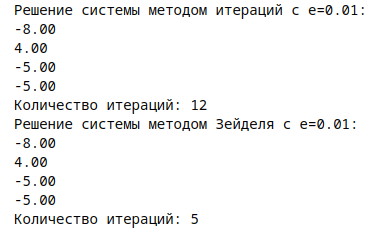
\includegraphics[width=.5\textwidth]{lab1.3}
\caption{Вывод в консоли}
\end{figure}
\pagebreak

\vfill

\subsection{Исходный код}

\lstinputlisting[title=\texttt{Lab1.3.cpp}]{../stud/saifullin/task1.3/Lab1.3.cpp}
\pagebreak
